\chapter{Casi d'uso}\label{sec:casi}
\section{Introduzione}
In questa sezione del documento vengono riportati tutti i casi d'uso relativi al prodotto del progetto.\\
Ogni caso d'uso sarà identificato da un codice alfanumerico, composto dall'acronimo "UC" di use case e seguito da dei numeri. Per ottenere una gerarchizzazione ad albero dei casi d'uso, con cui segnalare un sotto caso d'uso di un altro, i numeri saranno seguiti da uno o più punti, con cui sarà facile identificare il sotto caso d'uso rispetto al suo padre.\\
Ogni use case sarà inoltre corredato dalle informazioni riguardanti descrizione generale, \emph{attore\ped{G}} principale, pre condizioni, post condizioni e scenario, oltre ad attori secondari, generalizzazioni ed estensioni qualora presenti.

\section{Attori}
A seguito della richiesta esplicita da parte del proponente di non implementare alcun meccanismo di autenticazione, non vengono distinti nell'analisi dei casi d'uso utenti autenticati o meno, né utenti amministratori.\\
Per questo motivo, l'unico attore principale di tutti i casi d'uso sarà un utente generico, definito "user" negli UML dei casi d'uso.\\
L'attore secondario, definito con l'acronimo \ccgloss{LLM}, identifica il modello large language che è alla base del funzionamento del chatbot e delle funzionalità che permettono l'interazione dell'utente con esso. Il modello è identificato come attore secondario, e non come parte del sistema stesso, in quanto non sarà allenato dal sistema né il sistema avrà alcun potere su di esso.

\begin{figure}[H]
    \centering
    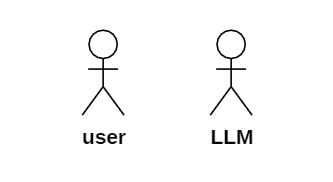
\includegraphics[width=0.4\linewidth]{Attori.PNG}
    \caption{Attori}
    \label{fig:attori}
\end{figure}

\newpage

\section{Elenco dei casi d'uso}

\subsection{UC-1 Visualizza interfaccia gestione documenti}
\begin{description}
    \item[Descrizione:] L’utente vuole accedere alla parte del sistema relativa alla gestione della documentazione.
    \item[Attore primario:] Utente generico.
    \item[Pre condizioni:]  Il sistema è stato inizializzato.
    \item[Post condizioni:] Il sistema mostra l’area di gestione dei documenti.
    \item[Scenario:] Il sistema è inizializzato e l’utente ha accesso all’interfaccia di gestione della documentazione.
\end{description}

\subsection{UC-2 Visualizza interfaccia chatbot}
\begin{description}
    \item[Descrizione:] L’utente vuole accedere alla parte del sistema relativa al chatbot.
    \item[Attore primario:] Utente generico.
    \item[Pre condizioni:] Il sistema è stato inizializzato.
    \item[Post condizioni:] Il sistema mostra l’interfaccia del chatbot.
    \item[Scenario:] Il sistema è inizializzato e l’utente ha accesso all’interfaccia del chatbot.
\end{description}

\begin{figure}[H]
    \centering
    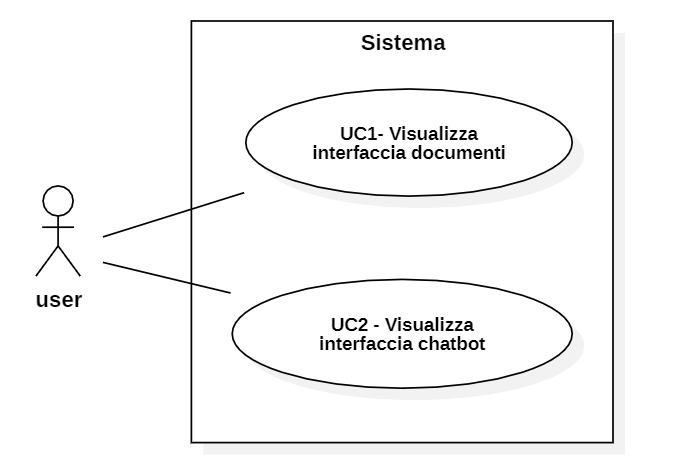
\includegraphics[width=0.7\linewidth]{UC1-2.PNG}
    \caption{Diagramma UML dei casi d'uso UC-1 e UC-2}
    \label{fig:UC1-2}
\end{figure}

\subsection{UC-3 Visualizza lista documenti}
\begin{description}
    \item[Descrizione:] L’utente vuole visualizzare la lista dei documenti presenti nel sistema.
    \item[Attore primario:] Utente generico.
    \item[Pre condizioni:] Il sistema mostra l’interfaccia di gestione documenti.
    \item[Post condizioni:] Il sistema mostra l’intera lista di documenti.
    \item[Scenario:] L’utente visualizza i documenti nella sezione di gestione dei documenti.
\end{description}

\begin{figure}[H]
    \centering
    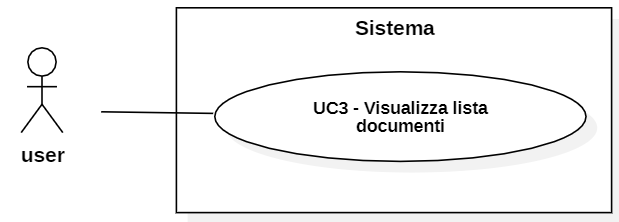
\includegraphics[width=0.8\linewidth]{UC3.PNG}
    \caption{Diagramma UML del caso d'uso UC-3}
    \label{fig:UC3}
\end{figure}

\subsection{UC-3.1 Visualizza singolo documento}
\begin{description}
    \item[Descrizione:] L'utente vuole visualizzare un particolare documento presente nel sistema.
    \item[Attore primario:] Utente generico.
    \item[Pre condizioni:] Il sistema mostra l’intera lista di documenti.
    \item[Post condizioni:] Il sistema mostra il documento di interesse.
    \item[Scenario:] L'utente visualizza il nome del documento;\\L'utente visualizza la data di inserimento del documento;\\L'utente visualizza i tag del documento;\\L'utente visualizza la preview del documento.
\end{description}

\begin{figure}[H]
    \centering
    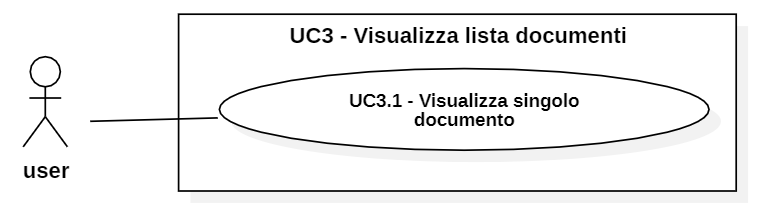
\includegraphics[width=0.8\linewidth]{UC3.1.PNG}
    \caption{Diagramma UML dei casi d'uso UC-3.1}
    \label{fig:UC3.1}
\end{figure}

\subsection{UC-3.1.1 Visualizza nome del documento}
\begin{description}
    \item[Descrizione:] L'utente vuole visualizzare il nome del documento di interesse.
    \item[Attore primario:] Utente generico.
    \item[Pre condizioni:] Il sistema mostra l’intera lista di documenti.
    \item[Post condizioni:] Il sistema mostra il nome del documento selezionato.
    \item[Scenario:] L'utente visualizza il nome del documento voluto.
\end{description}

\subsection{UC-3.1.2 Visualizza data di inserimento del documento}
\begin{description}
    \item[Descrizione:] L'utente vuole visualizzare la data di inserimento del documento di interesse.
    \item[Attore primario:] Utente generico.
    \item[Pre condizioni:] Il sistema mostra l’intera lista di documenti.
    \item[Post condizioni:] Il sistema mostra la data di inserimento del documento selezionato.
    \item[Scenario:] L'utente visualizza la data di inserimento del documento voluto.
\end{description}

\subsection{UC-3.1.3 Visualizza tag del documento}
\begin{description}
    \item[Descrizione:] L'utente vuole visualizzare i tag applicati al documento di interesse.
    \item[Attore primario:] Utente generico.
    \item[Pre condizioni:] Il sistema mostra l’intera lista di documenti.
    \item[Post condizioni:] Il sistema mostra i tag del documento selezionato.
    \item[Scenario:] L'utente visualizza i tag applicati al documento voluto.
\end{description}

\subsection{UC-3.1.4 Visualizza preview del documento}
\begin{description}
    \item[Descrizione:] L'utente vuole visualizzare il documento di interesse.
    \item[Attore primario:] Utente generico.
    \item[Pre condizioni:] Il sistema mostra l’intera lista di documenti.
    \item[Post condizioni:] Il sistema mostra il preview del documento selezionato.
    \item[Scenario:] L'utente visualizza il preview del documento voluto.
\end{description}

\begin{figure}[H]
    \centering
    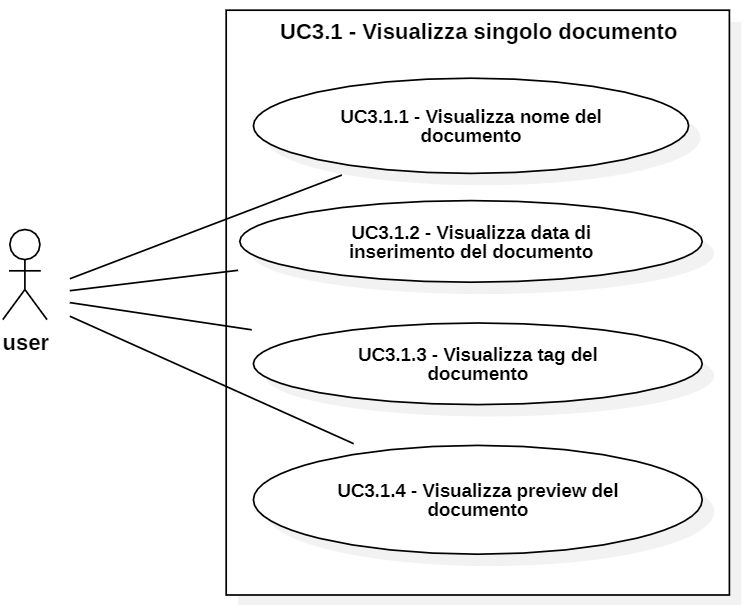
\includegraphics[width=0.8\linewidth]{UC3.1.1-2-3-4.PNG}
    \caption{Diagramma UML dei casi d'uso UC-3.1.1, UC-3.1.2, UC-3.1.3 e UC-3.1.4}
    \label{fig:UC3.1.1-2-3-4}
\end{figure}

\subsection{UC-4 Ricerca documento}
\begin{description}
    \item[Descrizione:] L’utente vuole poter ricercare un documento per nome, tag e/o data di inserimento.
    \item[Attore primario:] Utente generico.
    \item[Pre condizioni:] Il sistema mostra l’intera lista di documenti.
    \item[Post condizioni:] Il sistema mostra la lista di documenti che soddisfano la ricerca.
    \item[Scenario:] L’utente inserisce il nome del file, il tag e/o la data di inserimento.
\end{description}

\begin{figure}[H]
    \centering
    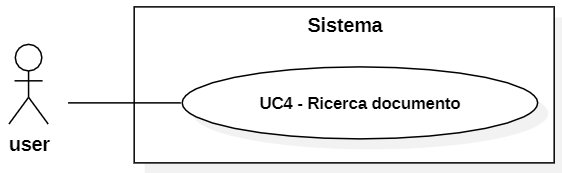
\includegraphics[width=0.8\linewidth]{UC4.PNG}
    \caption{Diagramma UML del caso d'uso UC-4}
    \label{fig:UC4}
\end{figure}

\subsection{UC-4.1 Ricerca documento per nome}
\begin{description}
    \item[Descrizione:] L’utente vuole poter ricercare un documento per nome.
    \item[Attore primario:] Utente generico.
    \item[Pre condizioni:] Il sistema mostra l’intera lista di documenti.
    \item[Post condizioni:] Il sistema mostra la lista di documenti che contengono il nome inserito.
    \item[Scenario:] L’utente inserisce il nome del file da cercare.
\end{description}

\subsection{UC-4.2 Ricerca documento per data}
\begin{description}
    \item[Descrizione:] L’utente vuole poter ricercare un documento per data di inserimento.
    \item[Attore primario:] Utente generico.
    \item[Pre condizioni:] Il sistema mostra l’intera lista di documenti.
    \item[Post condizioni:] Il sistema mostra la lista di documenti che sono stati inseriti dopo una certa data.
    \item[Scenario:] L’utente inserisce la data da cercare.
\end{description}

\subsection{UC-4.3 Ricerca documento per tag}
\begin{description}
    \item[Descrizione:] L’utente vuole poter ricercare un documento per il proprio tag.
    \item[Attore primario:] Utente generico.
    \item[Pre condizioni:] Il sistema mostra l’intera lista di documenti.
    \item[Post condizioni:] Il sistema mostra la lista di documenti che hanno quel tag.
    \item[Scenario:] L’utente inserisce il tag da cercare.
\end{description}

\begin{figure}[H]
    \centering
    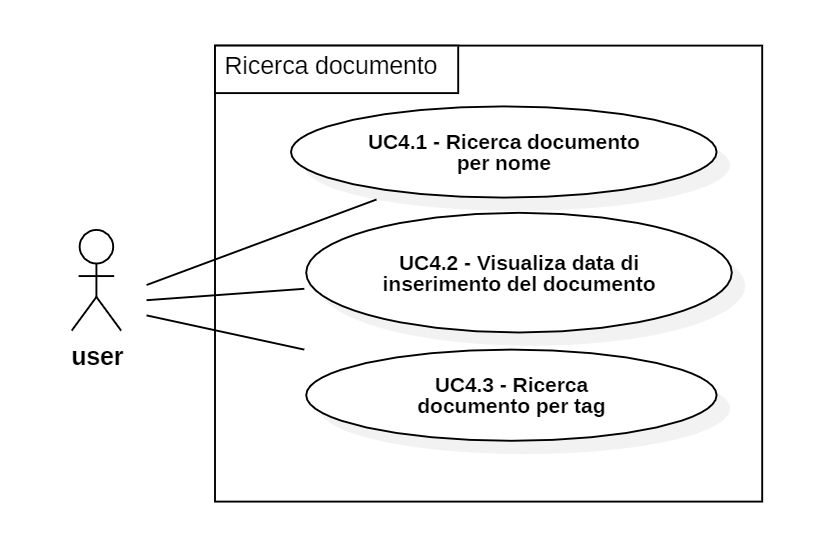
\includegraphics[width=0.8\linewidth]{UC4.1-2-3.PNG}
    \caption{Diagramma UML dei casi d'uso UC-4.1, UC-4.2 e UC-4.3}
    \label{fig:UC4.1-2-3}
\end{figure}

\subsection{UC-5 Aggiungi tag al documento}
\begin{description}
    \item[Descrizione:] L’utente vuole poter aggiungere un tag ad un documento.
    \item[Attore primario:] Utente generico.
    \item[Pre condizioni:] Il documento non ha il tag voluto dall’utente.
    \item[Post condizioni:] Il documento ha il nuovo tag selezionato dall’utente.
    \item[Scenario:] L’utente seleziona il documento;\\L’utente visualizza la lista di tag;\\L’utente seleziona il tag da aggiungere.
\end{description}

\begin{figure}[H]
    \centering
    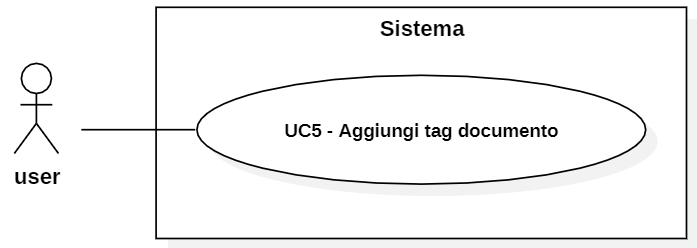
\includegraphics[width=0.8\linewidth]{UC5.PNG}
    \caption{Diagramma UML del caso d'uso UC-5}
    \label{fig:UC5}
\end{figure}

\subsection{UC-6 Rimuovi tag dal documento}
\begin{description}
    \item[Descrizione:] L’utente vuole poter rimuovere un tag da un documento.
    \item[Attore primario:] Utente generico.
    \item[Pre condizioni:] Il documento ha associato il tag non più voluto dall’utente.
    \item[Post condizioni:] Il documento non ha più associato il tag non voluto dall’utente.
    \item[Scenario:] L’utente seleziona il documento;\\L’utente visualizza la lista di tag associati a quel documento;\\L’utente seleziona il tag da rimuovere.
\end{description}

\begin{figure}[H]
    \centering
    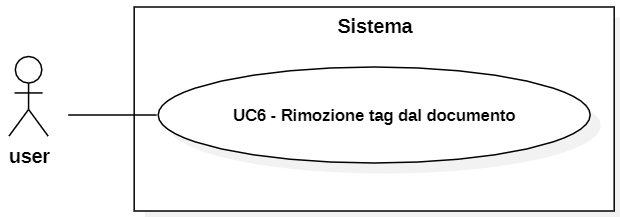
\includegraphics[width=0.8\linewidth]{UC6.PNG}
    \caption{Diagramma UML del caso d'uso UC-6}
    \label{fig:UC6}
\end{figure}

\subsection{UC-7 Creazione nuovo tag}
\begin{description}
    \item[Descrizione:] L’utente vuole poter creare un tag da poter associare ad un documento.
    \item[Attore primario:] Utente generico.
    \item[Pre condizioni:] Il sistema non presenta il nuovo tag voluto dall’utente.
    \item[Post condizioni:] Il sistema presenta il tag voluto dall’utente.
    \item[Scenario:] L’utente inserisce il nome del tag;\\L’utente inserisce il colore del tag.
\end{description}

\begin{figure}[H]
    \centering
    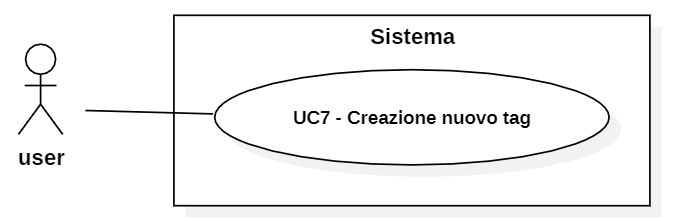
\includegraphics[width=0.8\linewidth]{UC7.PNG}
    \caption{Diagramma UML del caso d'uso UC-7}
    \label{fig:UC7}
\end{figure}

\subsection{UC-7.1 Aggiungi nome del tag}
\begin{description}
    \item[Descrizione:] L’utente vuole poter aggiungere un nome nella creazione del tag.
    \item[Attore primario:] Utente generico.
    \item[Pre condizioni:] Il sistema non conosce il nome  il tag voluto dall’utente e il nome associato.
    \item[Post condizioni:] Il sistema conosce il nome del tag voluto dall’utente.
    \item[Scenario:] L’utente inserisce il nome del tag.
\end{description}

\subsection{UC-7.2 Aggiungi colore del tag}
\begin{description}
    \item[Descrizione:] L’utente vuole poter aggiungere un colore nella creazione del tag.
    \item[Attore primario:] Utente generico.
    \item[Pre condizioni:] Il sistema non conosce il colore il tag voluto dall’utente.
    \item[Post condizioni:] Il sistema conosce il tag voluto dall’utente.
    \item[Scenario:] L’utente inserisce il colore del tag.
\end{description}

\subsection{UC-7.3 Aggiungi descrizione del tag}
\begin{description}
    \item[Descrizione:] L’utente vuole poter aggiungere una descrizione opzionale nella creazione del tag.
    \item[Attore primario:] Utente generico.
    \item[Pre condizioni:] Il sistema non conosce la descrizione  del tag voluto dall’utente.
    \item[Post condizioni:] Il sistema conosce la descrizione del tag voluto dall’utente.
    \item[Scenario:] L’utente inserisce la descrizione del tag.
\end{description}
\begin{figure}[H]
    \centering
    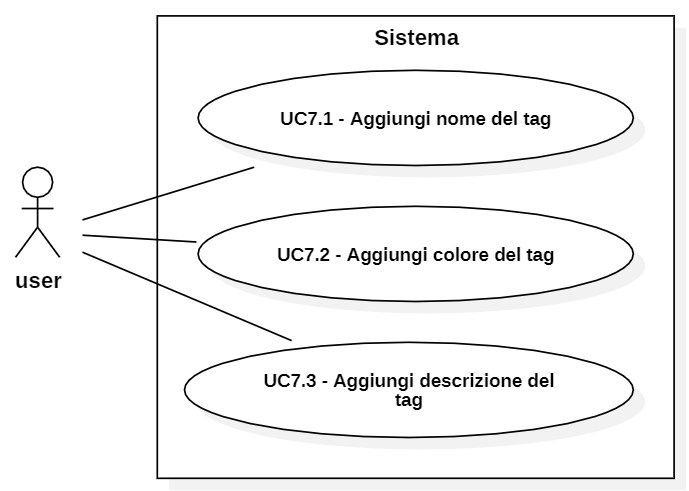
\includegraphics[width=0.8\linewidth]{UC7.1-2-3.PNG}
    \caption{Diagramma UML dei casi d'uso UC-7.1, UC-7.2 e UC-7.3}
    \label{fig:UC7.1-2-3}
\end{figure}

\subsection{UC-8 Visualizza lista tag}
\begin{description}
    \item[Descrizione:] L’utente vuole poter visualizzare la lista di tutti i tag creati.
    \item[Attore primario:] Utente generico.
    \item[Pre condizioni:] Il sistema mostra l'interfaccia di gestione dei documenti.
    \item[Post condizioni:] Il sistema mostra la lista dei tag creati.
    \item[Scenario:] L'utente visualizza ogni tag creato;\\L'utente visualizza il singolo tag creato.
\end{description}
\begin{figure}[H]
    \centering
    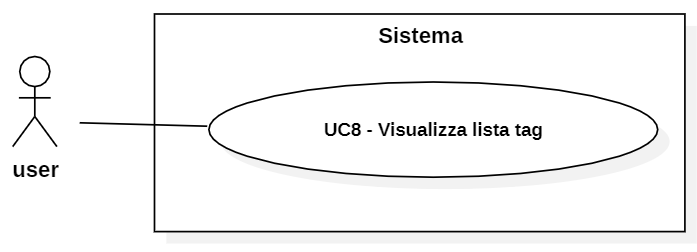
\includegraphics[width=0.8\linewidth]{UC8.PNG}
    \caption{Diagramma UML del caso d'uso UC-8}
    \label{fig:UC8}
\end{figure}

\subsection{UC-8.1 Visualizza singolo tag}
\begin{description}
    \item[Descrizione:] L’utente vuole poter visualizzare uno dei tag creati.
    \item[Attore primario:] Utente generico.
    \item[Pre condizioni:] Il sistema mostra la lista dei tag creati.
    \item[Post condizioni:] Il sistema mostra il tag di interesse.
    \item[Scenario:] L'utente visualizza il nome del tag;\\L'utente visualizza il colore del tag;\\L'utente visualizza la descrizione del tag.
\end{description}

\begin{figure}[H]
    \centering
    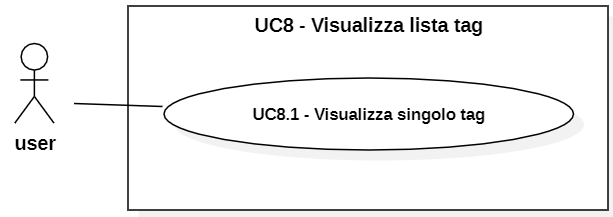
\includegraphics[width=0.8\linewidth]{UC8.1.PNG}
    \caption{Diagramma UML del caso d'uso UC-8.1}
    \label{fig:UC8.10}
\end{figure}
\subsection{UC-8.1.1 Visualizza nome del tag}
\begin{description}
    \item[Descrizione:] L’utente vuole poter visualizzare il nome del tag di interesse.
    \item[Attore primario:] Utente generico.
    \item[Pre condizioni:] Il sistema mostra la lista dei tag creati.
    \item[Post condizioni:] Il sistema mostra il nome del tag selezionato.
    \item[Scenario:] L'utente visualizza il nome del tag selezionato.
\end{description}

\subsection{UC-8.1.2 Visualizza colore del tag}
\begin{description}
    \item[Descrizione:] L’utente vuole poter visualizzare il colore del tag di interesse.
    \item[Attore primario:] Utente generico.
    \item[Pre condizioni:] Il sistema mostra la lista dei tag creati.
    \item[Post condizioni:] Il sistema mostra il colore del tag selezionato.
    \item[Scenario:] L'utente visualizza il colore del tag selezionato.
\end{description}

\subsection{UC-8.1.3 Visualizza descrizione del tag}
\begin{description}
    \item[Descrizione:] L’utente vuole poter visualizzare la descrizione del tag di interesse.
    \item[Attore primario:] Utente generico.
    \item[Pre condizioni:] Il sistema mostra la lista dei tag creati.
    \item[Post condizioni:] Il sistema mostra la descrizione del tag selezionato.
    \item[Scenario:] L'utente visualizza la descrizione del tag selezionato.
\end{description}

\begin{figure}[H]
    \centering
    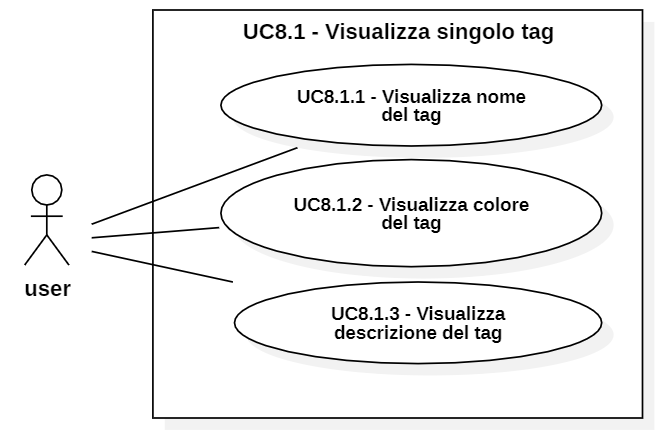
\includegraphics[width=0.8\linewidth]{UC8.1.1-2-3.PNG}
    \caption{Diagramma UML dei casi d'uso UC-8.1.1, UC-8.1.2 e UC-8.1.3}
    \label{fig:UC8.1.1-2-3}
\end{figure}

\subsection{UC-9 Elimina tag}
\begin{description}
    \item[Descrizione:] L'utente vuole eliminare uno dei tag presenti nel sistema.
    \item[Attore primario:] Utente generico.
    \item[Pre condizioni:] Il sistema presenta il tag non desiderato.
    \item[Post condizioni:] Il sistema non presenta più il tag indesiderato.
    \item[Scenario:] L'utente elimina uno dei tag presenti nel sistema.
\end{description}

\begin{figure}[H]
    \centering
    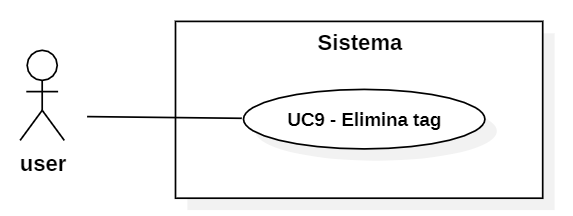
\includegraphics[width=0.8\linewidth]{UC9.PNG}
    \caption{Diagramma UML del caso d'uso UC-9}
    \label{fig:UC9}
\end{figure}

\subsection{UC-10 Elimina documento}
\begin{description}
    \item[Descrizione:] L'utente vuole eliminare uno dei documenti presenti nel sistema.
    \item[Attore primario:] Utente generico.
    \item[Pre condizioni:] Il sistema presenta il documento non desiderato.
    \item[Post condizioni:] Il sistema non presenta più il documento indesiderato.
    \item[Scenario:] L'utente elimina il documento di interesse;\\L'utente conferma l'eliminazione del documento dal sistema.
    \item[Scenario alternativo:] Visualizza errore nell'eliminazione di un documento (UC-11).
\end{description}

\subsection{UC-10.1 Conferma eliminazione documento}
\begin{description}
    \item[Descrizione:] L'utente vuole confermare l'eliminazione di uno dei documenti presenti nel sistema.
    \item[Attore primario:] Utente generico.
    \item[Pre condizioni:] Il sistema presenta il documento non desiderato.
    \item[Post condizioni:] Il sistema non presenta più il documento indesiderato.
    \item[Scenario:] L'utente conferma l'eliminazione del documento dal sistema.
\end{description}

\subsection{UC-11 Visualizza errore eliminazione documento}
\begin{description}
    \item[Descrizione:] L'utente visualizza un messaggio che lo notifica che c'è stato un errore nell'eliminazione di un documento.
    \item[Attore primario:] Utente generico
    \item[Pre condizioni:] L'utente tenta di eliminare un documento
    \item[Post condizioni:] Il sistema notifica un messaggio di errore e il documento non viene eliminato.
    \item[Scenario:] 
\end{description}

\begin{figure}[H]
    \centering
    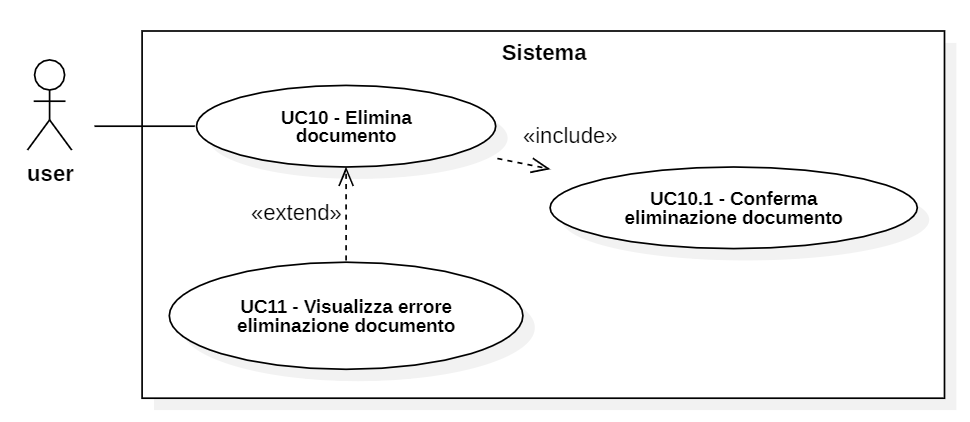
\includegraphics[width=0.8\linewidth]{UC10-11.png}
    \caption{Diagramma UML dei casi d'uso UC-10, UC-10.1 e UC-11}
    \label{fig:UC10-11}
\end{figure}

\subsection{UC-12 Aggiungi documento}
\begin{description}
    \item[Descrizione:] L'utente vuole aggiungere un documento nel sistema.
    \item[Attore primario:] Utente generico.
    \item[Pre condizioni:] Il sistema non presenta il documento di interesse.
    \item[Post condizioni:] Nel sistema è presente un nuovo documento.
    \item[Scenario:] L'utente aggiunge un nuovo documento tramite trascinamento o tramite file system.
    \item[Generalizzazioni:] Aggiungi documento tramite trascinamento (UC-12.1);\\Aggiungi documento tramite file system (UC-12.2).
    \item[Scenario alternativo:] Visualizza errore nell'inserimento di un documento (UC-13).
\end{description}

\subsection{UC-12.1 Aggiungi documento tramite trascinamento}
\begin{description}
    \item[Descrizione:] L'utente vuole aggiungere un documento nel sistema tramite trascinamento.
    \item[Attore primario:] Utente generico.
    \item[Pre condizioni:] Il sistema non presenta il documento di interesse.
    \item[Post condizioni:] Nel sistema è presente un nuovo documento.
    \item[Scenario:] L'utente aggiunge un nuovo documento nel sistema tramite trascinamento.
\end{description}

\subsection{UC-12.2 Aggiungi documento tramite file system}
\begin{description}
    \item[Descrizione:] L'utente vuole aggiungere un documento nel sistema tramite navigazione del file system.
    \item[Attore primario:] Utente generico.
    \item[Pre condizioni:] Il sistema non presenta il documento di interesse.
    \item[Post condizioni:] Nel sistema è presente un nuovo documento.
    \item[Scenario:] L'utente aggiunge un nuovo documento nel sistema tramite navigazione del file system.
\end{description}

\subsection{UC-13 Visualizza errore inserimento documento}
\begin{description}
    \item[Descrizione:] L'utente ha tentato di aggiungere nel sistema un documento che non può essere inserito, e visualizza un messaggio di errore.
    \item[Attore primario:] Utente generico.
    \item[Pre condizioni:] L'utente tenta di inserire un documento nel sistema.
    \item[Post condizioni:] Il sistema notifica un messaggio di errore e il documento non viene inserito nel sistema.
    \item[Scenario:] L'utente visualizza un messaggio di errore, a seguito di un tentativo di aggiungere un nuovo documento a sistema con un nome già in uso o di un formato non supportato o un file corrotto.
    \item[Generalizzazioni:] Visualizza errore nome file già presente (UC-12.1);\\Visualizza errore formato file (UC-12.2);\\Visualizza errore file corrotto (UC-12.3).
\end{description}

\subsection{UC-13.1 Visualizza errore nome file già presente}
\begin{description}
    \item[Descrizione:] Viene visualizzato un messaggio di errore per aver tentato di inserire un documento con un nome già in uso.
    \item[Attore primario:] Utente generico.
    \item[Pre condizioni:] L'utente tenta di inserire nel sistema un documento con un nome già in uso.
    \item[Post condizioni:] Il sistema notifica un messaggio di errore e il documento non viene inserito nel sistema.
    \item[Scenario:] L'utente visualizza un messaggio di errore, a seguito di un tentativo di aggiungere un nuovo documento a sistema con un nome già in uso.
\end{description}

\subsection{UC-13.2 Visualizza errore formato file}
\begin{description}
    \item[Descrizione:] Viene visualizzato un messaggio di errore per aver tentato di inserire un documento con un formato non supportato.
    \item[Attore primario:] Utente generico.
    \item[Pre condizioni:] L'utente tenta di inserire nel sistema un documento con un formato non supportato.
    \item[Post condizioni:] Il sistema notifica un messaggio di errore e il documento non viene inserito nel sistema.
    \item[Scenario:] L'utente visualizza un messaggio di errore, a seguito di un tentativo di aggiungere un nuovo documento a sistema con un formato non supportato.
\end{description}

\subsection{UC-13.3 Visualizza errore file corrotto}
\begin{description}
    \item[Descrizione:] Viene visualizzato un messaggio di errore per aver tentato di inserire un file corrotto.
    \item[Attore primario:] Utente generico.
    \item[Pre condizioni:] L'utente tenta di inserire nel sistema un documento in un file corrotto.
    \item[Post condizioni:] Il sistema notifica un messaggio di errore e il documento non viene inserito nel sistema.
    \item[Scenario:] L'utente visualizza un messaggio di errore, a seguito di un tentativo di aggiungere un nuovo documento a sistema tramite un file corrotto.
\end{description}

\begin{figure}[H]
    \centering
    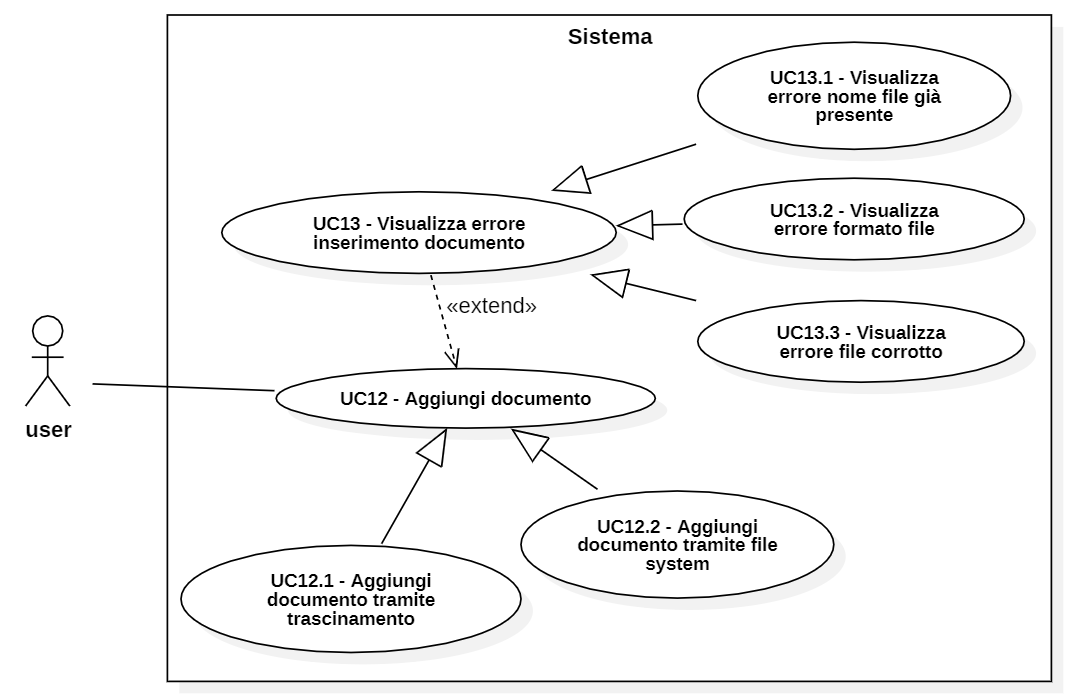
\includegraphics[width=\linewidth]{UC12-13.PNG}
    \caption{Diagramma UML dei casi d'uso UC-12, UC-12.1, UC-12.2, UC-13, UC-13.1, UC-13.2 e UC-13.3}
    \label{fig:UC12-13}
\end{figure}

\subsection{UC-14 Visualizza lista lingue chatbot}
\begin{description}
    \item[Descrizione:] L'utente vuole visualizzare la lista delle lingue supportate dal chatbot.
    \item[Attore primario:] Utente generico.
    \item[Pre condizioni:] Il sistema mostra l'interfaccia del chatbot.
    \item[Post condizioni:] Il sistema mostra la lista delle lingue supportate.
    \item[Scenario:] L'utente visualizza tutte le lingue utilizzabili nell'interfaccia del chatbot.
\end{description}

\begin{figure}[H]
    \centering
    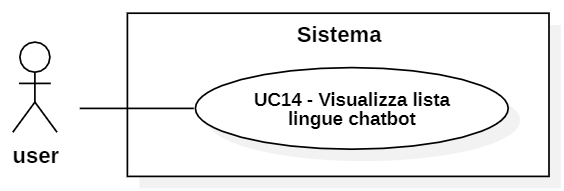
\includegraphics[width=0.8\linewidth]{UC14.png}
    \caption{Diagramma UML del caso d'uso UC-14}
    \label{fig:UC14}
\end{figure}

\subsection{UC-15 Seleziona lingua del chatbot}
\begin{description}
    \item[Descrizione:] L'utente vuole selezionare la lingua del sistema.
    \item[Attore primario:] Utente generico.
    \item[Pre condizioni:] Il sistema mostra la lista delle lingue supportate.
    \item[Post condizioni:] Il sistema aggiorna la lingua del chatbot.
    \item[Scenario:] L'utente visualizza la lista delle lingue del chatbot;\\L'utente seleziona una delle lingua disponibili.
\end{description}

\begin{figure}[H]
    \centering
    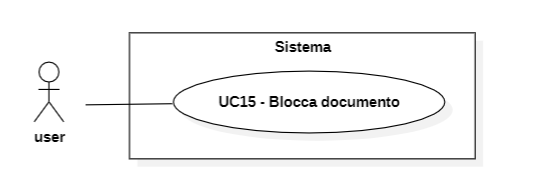
\includegraphics[width=0.8\linewidth]{UC15.png}
    \caption{Diagramma UML del caso d'uso UC-15}
    \label{fig:UC15}
\end{figure}

\subsection{UC-16 Inserisci domanda}
\begin{description}
    \item[Descrizione:] L'utente vuole inserire una domanda per il chatbot.
    \item[Attore primario:] Utente generico.
    \item[Pre condizioni:] Il sistema mostra l'interfaccia del chatbot.
    \item[Post condizioni:] Il sistema presenta la domanda dell'utente nello spazio relativo.
    \item[Scenario:] L'utente inserisce la domanda da rivolgere al sistema digitandola o attraverso un input vocale.
    \item[Generalizzazioni:] Digita domanda (UC-15.1);\\Input vocale della domanda (UC-15.2) 
\end{description}

\subsection{UC-16.1 Digita domanda}
\begin{description}
    \item[Descrizione:] L'utente vuole digitare la domanda da porgere al chatbot.
    \item[Attore primario:] Utente generico.
    \item[Pre condizioni:] Il sistema mostra l'interfaccia del chatbot.
    \item[Post condizioni:] Il sistema presenta la domanda digitata dall'utente nello spazio relativo.
    \item[Scenario:] L'utente inserisce la domanda da rivolgere al sistema digitandola.
\end{description}

\subsection{UC-16.2 Input vocale della domanda}
\begin{description}
    \item[Descrizione:] L'utente vuole inserire tramite microfono la domanda da porgere al sistema.
    \item[Attore primario:] Utente generico.
    \item[Pre condizioni:] Il sistema mostra l'interfaccia del chatbot.
    \item[Post condizioni:] Il sistema presenta la domanda posta a voce dall'utente nello spazio relativo.
    \item[Scenario:] L'utente inserisce la domanda da rivolgere al chatbot tramite input vocale.
    \item[Scenario alternativo:] Visualizza errore nell'inserimento della domanda tramite input vocale (UC-16).
\end{description}

\subsection{UC-17 Visualizza errore input vocale}
\begin{description}
    \item[Descrizione:] L'utente ha tentato di inserire senza successo la domanda da porre al sistema tramite input vocale.
    \item[Attore primario:] Utente generico.
    \item[Pre condizioni:] L'utente tenta di inserire la domanda tramite input vocale.
    \item[Post condizioni:] Il sistema non presenta la domanda posta a voce dall'utente nello spazio relativo.
    \item[Scenario:] L'utente visualizza un messaggio di errore, a seguito di un tentativo fallito di inserire tramite voce la domanda da porre al sistema.
\end{description}

\begin{figure}[H]
    \centering
    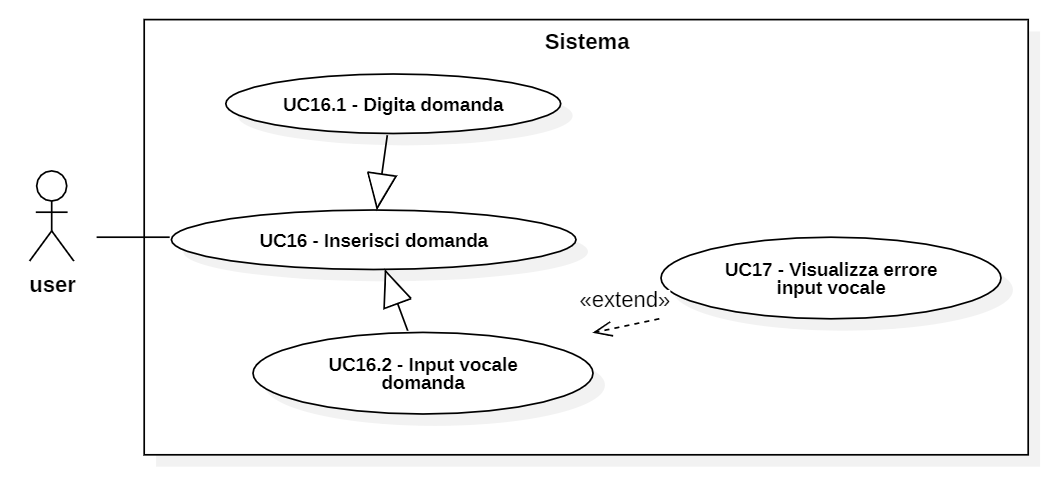
\includegraphics[width=\linewidth]{UC16-17.PNG}
    \caption{Diagramma UML dei casi d'uso UC-16, UC-16.1, UC-16.2 e UC-17}
    \label{fig:UC16-17}
\end{figure}

\subsection{UC-18 Invia domanda}
\begin{description}
    \item[Descrizione:] L'utente vuole inviare una domanda al sistema.
    \item[Attore primario:] Utente generico.
    \item[Pre condizioni:] Il sistema presenta la domanda posta dall'utente.
    \item[Post condizioni:] Il sistema ha processato correttamente la domanda inserita dall'utente.
    \item[Scenario:] L'utente seleziona l'invio della domanda al sistema.
    \item[Scenario alternativo:] Visualizza errore invio domanda (UC-19).
\end{description}

\subsection{UC-19 Visualizza errore invio domanda}
\begin{description}
    \item[Descrizione:] L'utente visualizza un messaggio che lo informa che c'è stato un errore nell'invio della domanda.
    \item[Attore primario:] Utente generico.
    \item[Pre condizioni:] L'utente ha tentato di inviare una domanda.
    \item[Post condizioni:] Il sistema notifica un messaggio di errore e non invia la domanda.
    \item[Scenario:] L'utente visualizza un messaggio di errore, a seguito di un tentativo di inviare una domanda.
\end{description}

\begin{figure}[H]
    \centering
    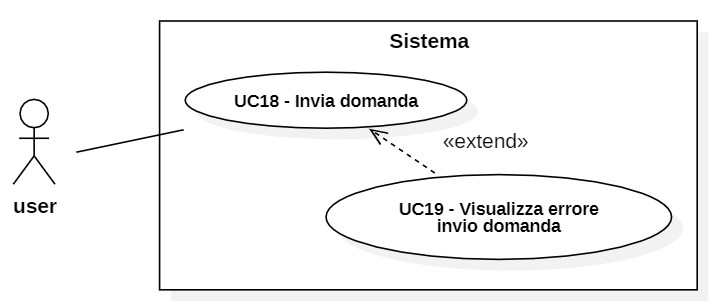
\includegraphics[width=\linewidth]{UC18-19.PNG}
    \caption{Diagramma UML dei casi d'uso UC-18 e UC-19}
    \label{fig:UC18-19}
\end{figure}

\subsection{UC-20 Visualizza risposta}
\begin{description}
    \item[Descrizione:] L'utente vuole visualizzare la risposta alla domanda che ha inviato in precedenza.
    \item[Attore primario:] Utente generico.
    \item[Attore secondario:] Modello LLM. 
    \item[Pre condizioni:] Il sistema ha ricevuto e processato la domanda posta dall'utente.
    \item[Post condizioni:] Il sistema restituisce una risposta all'utente.
    \item[Scenario:] L'utente inserisce una domanda;\\L'utente invia una domanda;\\L'utente visualizza la risposta alla domanda posta al sistema.
    \item[Scenario alternativo:] UC-21
\end{description}

\subsection{UC-21 Visualizza errore risposta}
\begin{description}
    \item[Descrizione:] L'utente visualizza un messaggio che lo informa che c'è stato un errore nel ricevere la risposta.
    \item[Attore primario:] Utente generico.
    \item[Pre condizioni:] 
    \item[Post condizioni:] Il sistema notifica un messaggio di errore e non restituisce la risposta.
    \item[Scenario:] 
\end{description}

\begin{figure}[H]
    \centering
    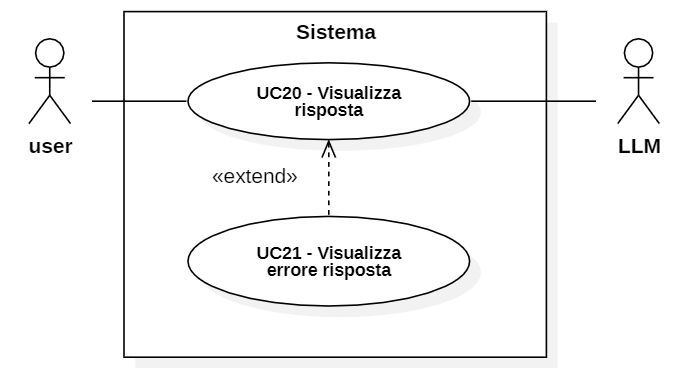
\includegraphics[width=0.8\linewidth]{UC20-21.PNG}
    \caption{Diagramma UML de casi d'uso UC-20 e UC-21}
    \label{fig:UC20-21}
\end{figure}

\subsection{UC-22 Crea nuova sessione}
\begin{description}
    \item[Descrizione:] L'utente vuole creare una nuova sessione di conversazione col chatbot.
    \item[Attore primario:] Utente generico.
    \item[Pre condizioni:] Il sistema non presenta la nuova sessione di interesse dell'utente.
    \item[Post condizioni:] Il sistema inizializza una nuova sessione.
    \item[Scenario:] L'utente crea una nuova sessione di conversazione nel sistema.
    \item[Scenario alternativo:] UC-23
\end{description}

\subsection{UC-23 Visualizza errore creazione sessione}
\begin{description}
    \item[Descrizione:] L'utente visualizza un messaggio che lo notifica che c'è stato un errore nella creazione di una nuova sessione.
    \item[Attore primario:] Utente generico.
    \item[Pre condizioni:] L'utente ha tentato di creare una nuova sessione.
    \item[Post condizioni:] Il sistema notifica un messaggio di errore e non crea una nuova sessione.
    \item[Scenario:] 
\end{description}

\begin{figure}[H]
    \centering
    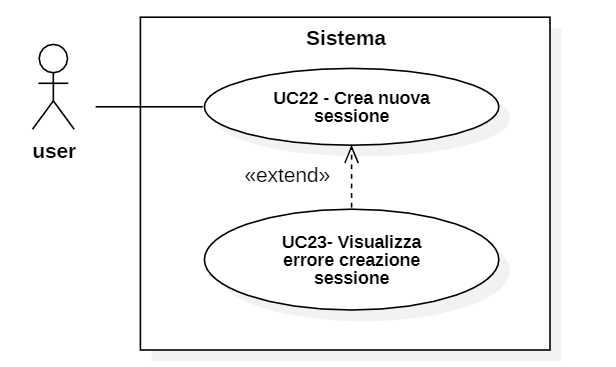
\includegraphics[width=0.8\linewidth]{UC22-23.PNG}
    \caption{Diagramma UML de casi d'uso UC-22 e UC-23}
    \label{fig:UC22-23}
\end{figure}

\subsection{UC-24 Visualizza lista sessioni aperte}
\begin{description}
    \item[Descrizione:] L'utente vuole visualizzare la lista delle sessioni di conversazione col chatbot aperte.
    \item[Attore primario:] Utente generico.
    \item[Pre condizioni:] Il sistema mostra l'interfaccia relativa al chatbot.
    \item[Post condizioni:] Il sistema mostra la lista delle sessioni attive.
    \item[Scenario:] L'utente visualizza la lista delle sessioni attive;\\L'utente visualizza una delle sessioni attive di conversazione col chatbot.
    \item[Scenario alternativo:] UC-25
\end{description}

\subsection{UC-24.1 Visualizza singola sessione}
\begin{description}
    \item[Descrizione:] L'utente vuole visualizzare una delle sessioni di conversazione col chatbot.
    \item[Attore primario:] Utente generico.
    \item[Pre condizioni:] Il sistema mostra la lista delle sessioni attive.
        \item[Post condizioni:] Il sistema mostra una particolare sessione attiva.
    \item[Scenario:] L'utente visualizza una delle sessioni attive nel sistema
\end{description}

\subsection{UC-25 Visualizza errore sessioni aperte }
\begin{description}
    \item[Descrizione:] L'utente visualizza un messaggio che lo notifica che c'è stato un errore nella visualizzazione delle sessioni aperte.
    \item[Attore primario:] Utente generico.
    \item[Pre condizioni:] Il sistema ha tentato di visualizzare le sessioni aperte.
    \item[Post condizioni:] Il sistema notifica un messaggio di errore e non visualizza le sessioni aperte.
    \item[Scenario:] 
\end{description}

\begin{figure}[H]
    \centering
    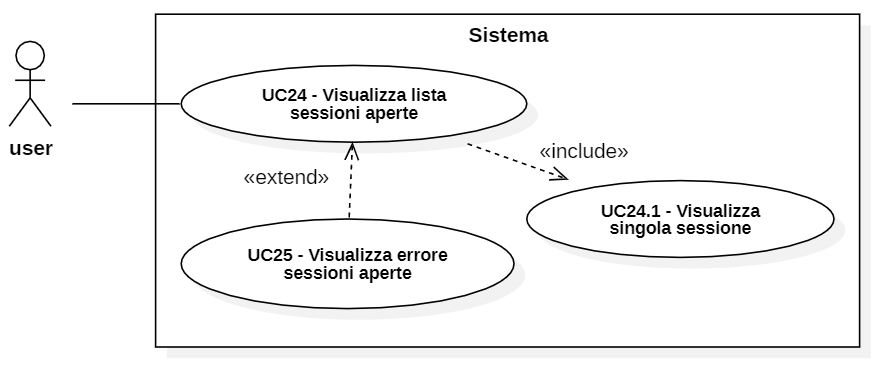
\includegraphics[width=0.8\linewidth]{UC24-25.PNG}
    \caption{Diagramma UML de casi d'uso UC-24, UC-24.1 e UC-25}
    \label{fig:UC24-25}
\end{figure}

\subsection{UC-26 Elimina sessione}
\begin{description}
    \item[Descrizione:] L'utente vuole eliminare una delle sessioni di conversazioni attive nel sistema.
    \item[Attore primario:] Utente generico.
    \item[Pre condizioni:] Il sistema presenta la sessione che l'utente vuole eliminare.
    \item[Post condizioni:] Il sistema non presenta più la sessione eliminata dall'utente.
    \item[Scenario:] L'utente elimina dal sistema la sessione di conversazione con il chatbot desiderata.
    \item[Scenario alternativo:] UC-27
\end{description}

\subsection{UC-27 Visualizza errore eliminazione sessione }
\begin{description}
    \item[Descrizione:] L'utente visualizza un messaggio che lo notifica che c'è stato un errore nell'eliminazione di una sessione.
    \item[Attore primario:] Utente generico.
    \item[Pre condizioni:] L'utente ha tentato di eliminare una sessione.
    \item[Post condizioni:] Il sistema notifica un messaggio di errore e non elimina la sessione.
    \item[Scenario:] 
\end{description}

\begin{figure}[H]
    \centering
    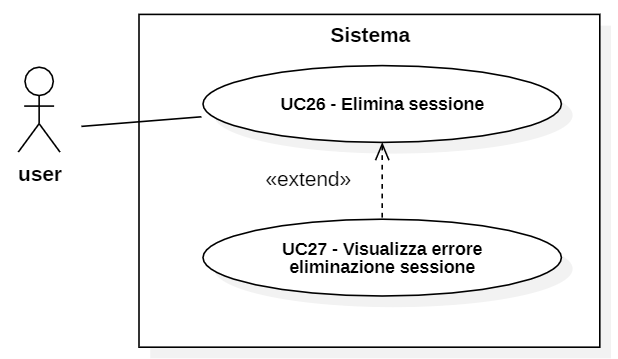
\includegraphics[width=0.9\linewidth]{UC26-27.PNG}
    \caption{Diagramma UML de casi d'uso UC-26 e UC-27}
    \label{fig:UC26-27}
\end{figure}

\subsection{UC-28 Visualizza chat history}
\begin{description}
    \item[Descrizione:] L'utente vuole visualizzare lo scambio di domande e risposte avvenuto in precedenza con il sistema in una sessione.
    \item[Attore primario:] Utente generico.
    \item[Pre condizioni:] Il sistema ha in precedenza ricevuto una o più domande a cui ha fornito risposte.
    \item[Post condizioni:] Il sistema mostra lo storico delle conversazioni dell'utente
    \item[Scenario:] L'utente visualizza lo scambio di domande e risposte in una sessione con il sistema.
    \item[Scenario alternativo:] UC-29
\end{description} 

\subsection{UC-29 Visualizza errore chat history }
\begin{description}
    \item[Descrizione:] L'utente visualizza un messaggio che lo notifica che c'è stato un errore nella visualizzazione della chat history.
    \item[Attore primario:] Utente generico.
    \item[Pre condizioni:] Il sistema ha tentato di visualizzare la chat history.
    \item[Post condizioni:] Il sistema notifica un messaggio di errore e non visualizza la chat history.
    \item[Scenario:] 
\end{description}

\begin{figure}[H]
    \centering
    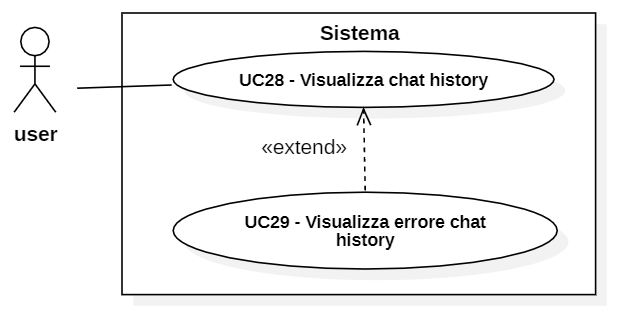
\includegraphics[width=0.9\linewidth]{UC28-29.PNG}
    \caption{Diagramma UML de casi d'uso UC-28 e UC-29}
    \label{fig:UC28-29}
\end{figure}

\subsection{UC-30 Elimina chat history}
\begin{description}
    \item[Descrizione:] L'utente vuole eliminare lo scambio di domande e risposte, avvenuto in precedenza con il chatbot, dalla sessione del sistema.
    \item[Attore primario:] Utente generico.
    \item[Pre condizioni:] Il sistema presenta la chat history.
    \item[Post condizioni:] Il sistema non presenta più alcuna chat history in quella sessione.
    \item[Scenario:] L'utente elimina la chat history della sessione corrente.
    \item[Scenario alternativo:] UC-31
\end{description}

\subsection{UC-31 Visualizza errore eliminazione chat history }
\begin{description}
    \item[Descrizione:] L'utente visualizza un messaggio che lo notifica che c'è stato un errore nell'eliminazione della chat history.
    \item[Attore primario:] Utente generico
    \item[Pre condizioni:] L'utente ha tentato di eliminare la chat history.
    \item[Post condizioni:] Il sistema notifica un messaggio di errore e non elimina la chat history.
    \item[Scenario:] 
\end{description}

\begin{figure}[H]
    \centering
    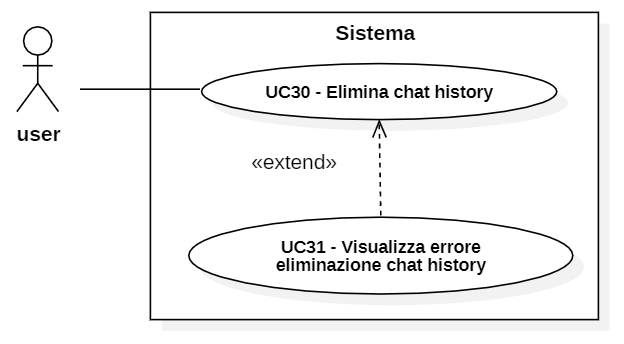
\includegraphics[width=0.9\linewidth]{UC30-31.PNG}
    \caption{Diagramma UML de casi d'uso UC-30 e UC-31}
    \label{fig:UC30-31}
\end{figure}

\subsection{UC-32 Visualizza informazioni risposta}
\begin{description}
    \item[Descrizione:] L'utente vuole visualizzare le informazioni del documento da cui deriva la risposta ricevuta.
    \item[Attore primario:] Utente generico.
    \item[Pre condizioni:] Il sistema mostra la risposta ad una domanda dell'utente.
    \item[Post condizioni:] Il sistema mostra le informazioni riguardanti la fonte della risposta.
    \item[Scenario:] L'utente inserisce una domanda.\\L'utente invia una domanda.\\L'utente visualizza una risposta.\\L'utente visualizza le informazioni sul documento fonte della risposta.
\end{description}

\begin{figure}[H]
    \centering
    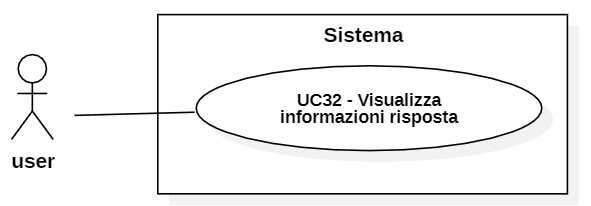
\includegraphics[width=0.9\linewidth]{UC32.PNG}
    \caption{Diagramma UML del caso d'uso UC-32}
    \label{fig:UC32}
\end{figure}

\subsection{UC-32.1 Visualizza nome del documento}
\begin{description}
    \item[Descrizione:] L'utente vuole poter visualizzare il nome del documento.
    \item[Attore primario:] Utente generico.
    \item[Attore secondario:] Modello LLM.
    \item[Pre condizioni:] Il sistema non visualizza il nome del documento.
    \item[Post condizioni:] Il sistema visualizza il nome del documento.
    \item[Scenario:] L'utente visualizza il nome del documento.
\end{description}

\subsection{UC-32.2 Visualizza pagina del documento}
\begin{description}
    \item[Descrizione:] L'utente vuole poter visualizzare la pagina del documento.
    \item[Attore primario:] Utente generico.
    \item[Attore secondario:] Modello LLM.
    \item[Pre condizioni:] Il sistema non visualizza la pagina del documento.
    \item[Post condizioni:] Il sistema visualizza la pagina del documento.
    \item[Scenario:] L'utente visualizza la pagina del documento.
\end{description}

\subsection{UC-32.3 Visualizza preview del documento}
\begin{description}
    \item[Descrizione:] L'utente vuole poter avere un preview del documento.
    \item[Attore primario:] Utente generico.
    \item[Pre condizioni:] Il sistema non presenta il preview del documento.
    \item[Post condizioni:] Il sistema visualizza il preview del documento.
    \item[Scenario:] L'utente seleziona il documento voluto. \\L'utente visualizza il documento.
\end{description}

\begin{figure}[H]
    \centering
    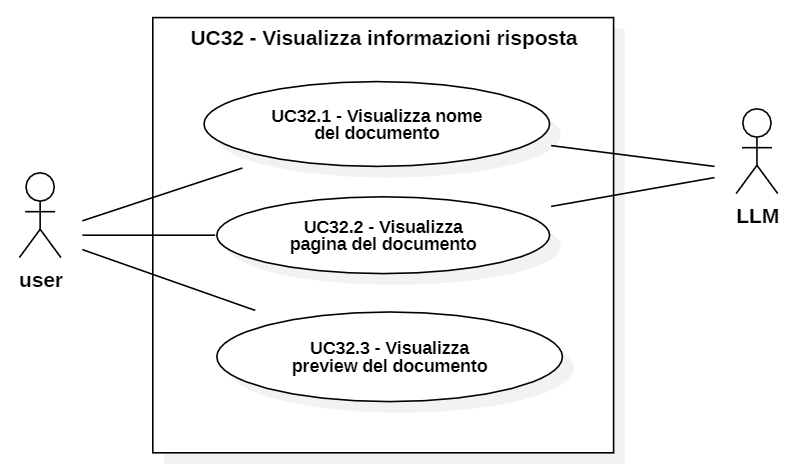
\includegraphics[width=0.9\linewidth]{UC32.1-2-3.PNG}
    \caption{Diagramma UML dei casi d'uso UC-32.1, UC-32.2 e UC-32.3}
    \label{fig:UC32.1-2-3}
\end{figure}

\subsection{UC-33 Ascolta risposta}
\begin{description}
    \item[Descrizione:] L'utente vuole sentire la lettura della risposta ricevuta.
    \item[Attore primario:] Utente generico.
    \item[Attore secondario:] Modello LLM.
    \item[Pre condizioni:] Il sistema mostra la risposta ad una domanda dell'utente.
    \item[Post condizioni:] Il sistema riproduce la risposta con un audio.
    \item[Scenario:] L'utente inserisce una domanda.\\L'utente invia una domanda.\\L'utente ascolta la risposta ricevuta dal sistema.
\end{description}

\begin{figure}[H]
    \centering
    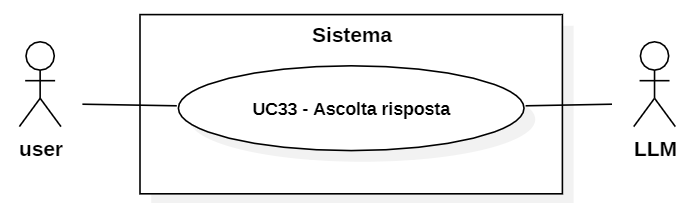
\includegraphics[width=0.9\linewidth]{UC33.PNG}
    \caption{Diagramma UML del caso d'uso UC-33}
    \label{fig:UC33}
\end{figure}
